
% LaTeX Beamer file automatically generated from DocOnce
% https://github.com/doconce/doconce

%-------------------- begin beamer-specific preamble ----------------------

\documentclass{beamer}

\usetheme{red_plain}
\usecolortheme{default}

% turn off the almost invisible, yet disturbing, navigation symbols:
\setbeamertemplate{navigation symbols}{}

% Examples on customization:
%\usecolortheme[named=RawSienna]{structure}
%\usetheme[height=7mm]{Rochester}
%\setbeamerfont{frametitle}{family=\rmfamily,shape=\itshape}
%\setbeamertemplate{items}[ball]
%\setbeamertemplate{blocks}[rounded][shadow=true]
%\useoutertheme{infolines}
%
%\usefonttheme{}
%\useinntertheme{}
%
%\setbeameroption{show notes}
%\setbeameroption{show notes on second screen=right}

% fine for B/W printing:
%\usecolortheme{seahorse}

\usepackage{pgf}
\usepackage{graphicx}
\usepackage{epsfig}
\usepackage{relsize}

\usepackage{fancybox}  % make sure fancybox is loaded before fancyvrb

\usepackage{fancyvrb}
%\usepackage{minted} % requires pygments and latex -shell-escape filename
%\usepackage{anslistings}
%\usepackage{listingsutf8}

\usepackage{amsmath,amssymb,bm}
%\usepackage[latin1]{inputenc}
\usepackage[T1]{fontenc}
\usepackage[utf8]{inputenc}
\usepackage{colortbl}
\usepackage[english]{babel}
\usepackage{tikz}
\usepackage{framed}
% Use some nice templates
\beamertemplatetransparentcovereddynamic

% --- begin table of contents based on sections ---
% Delete this, if you do not want the table of contents to pop up at
% the beginning of each section:
% (Only section headings can enter the table of contents in Beamer
% slides generated from DocOnce source, while subsections are used
% for the title in ordinary slides.)
\AtBeginSection[]
{
  \begin{frame}<beamer>[plain]
  \frametitle{}
  %\frametitle{Outline}
  \tableofcontents[currentsection]
  \end{frame}
}
% --- end table of contents based on sections ---

% If you wish to uncover everything in a step-wise fashion, uncomment
% the following command:

%\beamerdefaultoverlayspecification{<+->}

\newcommand{\shortinlinecomment}[3]{\note{\textbf{#1}: #2}}
\newcommand{\longinlinecomment}[3]{\shortinlinecomment{#1}{#2}{#3}}

\definecolor{linkcolor}{rgb}{0,0,0.4}
\hypersetup{
    colorlinks=true,
    linkcolor=linkcolor,
    urlcolor=linkcolor,
    pdfmenubar=true,
    pdftoolbar=true,
    bookmarksdepth=3
    }
\setlength{\parskip}{0pt}  % {1em}

\newenvironment{doconceexercise}{}{}
\newcounter{doconceexercisecounter}
\newenvironment{doconce:movie}{}{}
\newcounter{doconce:movie:counter}

\newcommand{\subex}[1]{\noindent\textbf{#1}}  % for subexercises: a), b), etc

%-------------------- end beamer-specific preamble ----------------------

% Add user's preamble




% insert custom LaTeX commands...

\raggedbottom
\makeindex

%-------------------- end preamble ----------------------

\begin{document}

% matching end for #ifdef PREAMBLE

\newcommand{\exercisesection}[1]{\subsection*{#1}}



% ------------------- main content ----------------------



% ----------------- title -------------------------

\title{Premio Nobel per la  Fisica 2024}

% ----------------- author(s) -------------------------

\author{Martino (Morten) Hjorth-Jensen, Dipartimento di Fisica, UniOslo, Oslo, Norvegia\inst{}}
\institute{}
% ----------------- end author(s) -------------------------

\date{UniTN, Dipartimento di Fisica, 9 dicembre 2024
\\ \ \\ 
\centerline{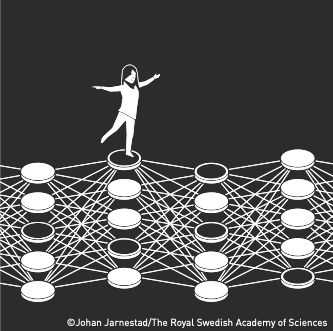
\includegraphics[width=0.45\linewidth]{figures/nnillustration.png}}
% <optional copyright>
}

\vspace{6mm}



\vspace{6mm}

\begin{frame}[plain,fragile]
\titlepage
\end{frame}

\begin{frame}[plain,fragile]
\frametitle{Nobel per la  Fisica  sull'apprendimento automatico}

\begin{block}{}
Quali furono le ragioni e motivazioni per dare  il premio Nobel per la Fisica a Hopfield e Hinton? 
\end{block}

\begin{block}{}
Tutto il materiale per questo seminario lo potete trovare sul sito  \href{{http://mhjensenseminars.github.io/MachineLearningTalk/doc/pub/UniTNDicembre2024/pdf/UniTNDicembre2024.pdf}}{\nolinkurl{http://mhjensenseminars.github.io/MachineLearningTalk/doc/pub/UniTNDicembre2024/pdf/UniTNDicembre2024.pdf}}
\end{block}
\end{frame}

\begin{frame}[plain,fragile]
\frametitle{Premio Nobel 2024}

Tratto dal sito per il premio Nobel:
\begin{block}{}
This year’s two Nobel Laureates in Physics have used tools from
physics to develop methods that are the foundation of today’s powerful
machine learning. John Hopfield created an associative memory that can
store and reconstruct images and other types of patterns in
data. Geoffrey Hinton invented a method that can autonomously find
properties in data, and so perform tasks such as identifying specific
elements in pictures.
\end{block}
\end{frame}

\begin{frame}[plain,fragile]
\frametitle{Geoffrey Hinton}

\href{{https://www.nobelprize.org/prizes/physics/2024/press-release/#:~:text=Geoffrey%20Hinton%20invented%20a%20method,learning%20using%20artificial%20neural%20networks}}{Dal sito per il premio Nobel}.
\begin{block}{}
Geoffrey Hinton used the Hopfield network as the foundation for a new
network that uses a different method: the Boltzmann machine. This can
learn to recognise characteristic elements in a given type of
data. Hinton used tools from statistical physics, the science of
systems built from many similar components. The machine is trained by
feeding it examples that are very likely to arise when the machine is
run. The Boltzmann machine can be used to classify images or create
new examples of the type of pattern on which it was trained. Hinton
has built upon this work, helping initiate the current explosive
development of machine learning.
\end{block}
\end{frame}

\begin{frame}[plain,fragile]
\frametitle{AI/ML and some statements you may have heard (and what do they mean?)}

\begin{enumerate}
\item Fei-Fei Li on ImageNet: \textbf{map out the entire world of objects} (\href{{https://cacm.acm.org/news/219702-the-data-that-transformed-ai-research-and-possibly-the-world/fulltext}}{The data that transformed AI research})

\item Russell and Norvig in their popular textbook: \textbf{relevant to any intellectual task; it is truly a universal field} (\href{{http://aima.cs.berkeley.edu/}}{Artificial Intelligence, A modern approach})

\item Woody Bledsoe puts it more bluntly: \textbf{in the long run, AI is the only science} (quoted in Pamilla McCorduck, \href{{https://www.pamelamccorduck.com/machines-who-think}}{Machines who think})
\end{enumerate}

\noindent
If you wish to have a critical read on AI/ML from a societal point of view, see \href{{https://www.katecrawford.net/}}{Kate Crawford's recent text Atlas of AI}. 

\textbf{Here: with AI/ML we intend a collection of machine learning methods with an emphasis on statistical learning and data analysis}
\end{frame}

\begin{frame}[plain,fragile]
\frametitle{Types of machine learning}

\begin{block}{}
The approaches to machine learning are many, but are often split into two main categories. 
In \emph{supervised learning} we know the answer to a problem,
and let the computer deduce the logic behind it. On the other hand, \emph{unsupervised learning}
is a method for finding patterns and relationship in data sets without any prior knowledge of the system.

An important  third category is  \emph{reinforcement learning}. This is a paradigm 
of learning inspired by behavioural psychology, where learning is achieved by trial-and-error, 
solely from rewards and punishment.
\end{block}
\end{frame}

\begin{frame}[plain,fragile]
\frametitle{Main categories}

\begin{block}{}
Another way to categorize machine learning tasks is to consider the desired output of a system.
Some of the most common tasks are:

\begin{itemize}
\item Classification: Outputs are divided into two or more classes. The goal is to   produce a model that assigns inputs into one of these classes. An example is to identify  digits based on pictures of hand-written ones. Classification is typically supervised learning.

\item Regression: Finding a functional relationship between an input data set and a reference data set.   The goal is to construct a function that maps input data to continuous output values.

\item Clustering: Data are divided into groups with certain common traits, without knowing the different groups beforehand.  It is thus a form of unsupervised learning.
\end{itemize}

\noindent
\end{block}
\end{frame}

\begin{frame}[plain,fragile]
\frametitle{The plethora  of machine learning algorithms/methods}

\begin{enumerate}
\item Deep learning: Neural Networks (NN), Convolutional NN, Recurrent NN, Boltzmann machines, autoencoders and variational autoencoders  and generative adversarial networks, stable diffusion and many more generative models

\item Bayesian statistics and Bayesian Machine Learning, Bayesian experimental design, Bayesian Regression models, Bayesian neural networks, Gaussian processes and much more

\item Dimensionality reduction (Principal component analysis), Clustering Methods and more

\item Ensemble Methods, Random forests, bagging and voting methods, gradient boosting approaches 

\item Linear and logistic regression, Kernel methods, support vector machines and more

\item Reinforcement Learning; Transfer Learning and more 
\end{enumerate}

\noindent
\end{frame}

\begin{frame}[plain,fragile]
\frametitle{Example of generative modeling, \href{{https://www.oreilly.com/library/view/generative-deep-learning/9781098134174/ch01.html}}{taken from Generative Deep Learning by David Foster}}

\vspace{6mm}

% inline figure
\centerline{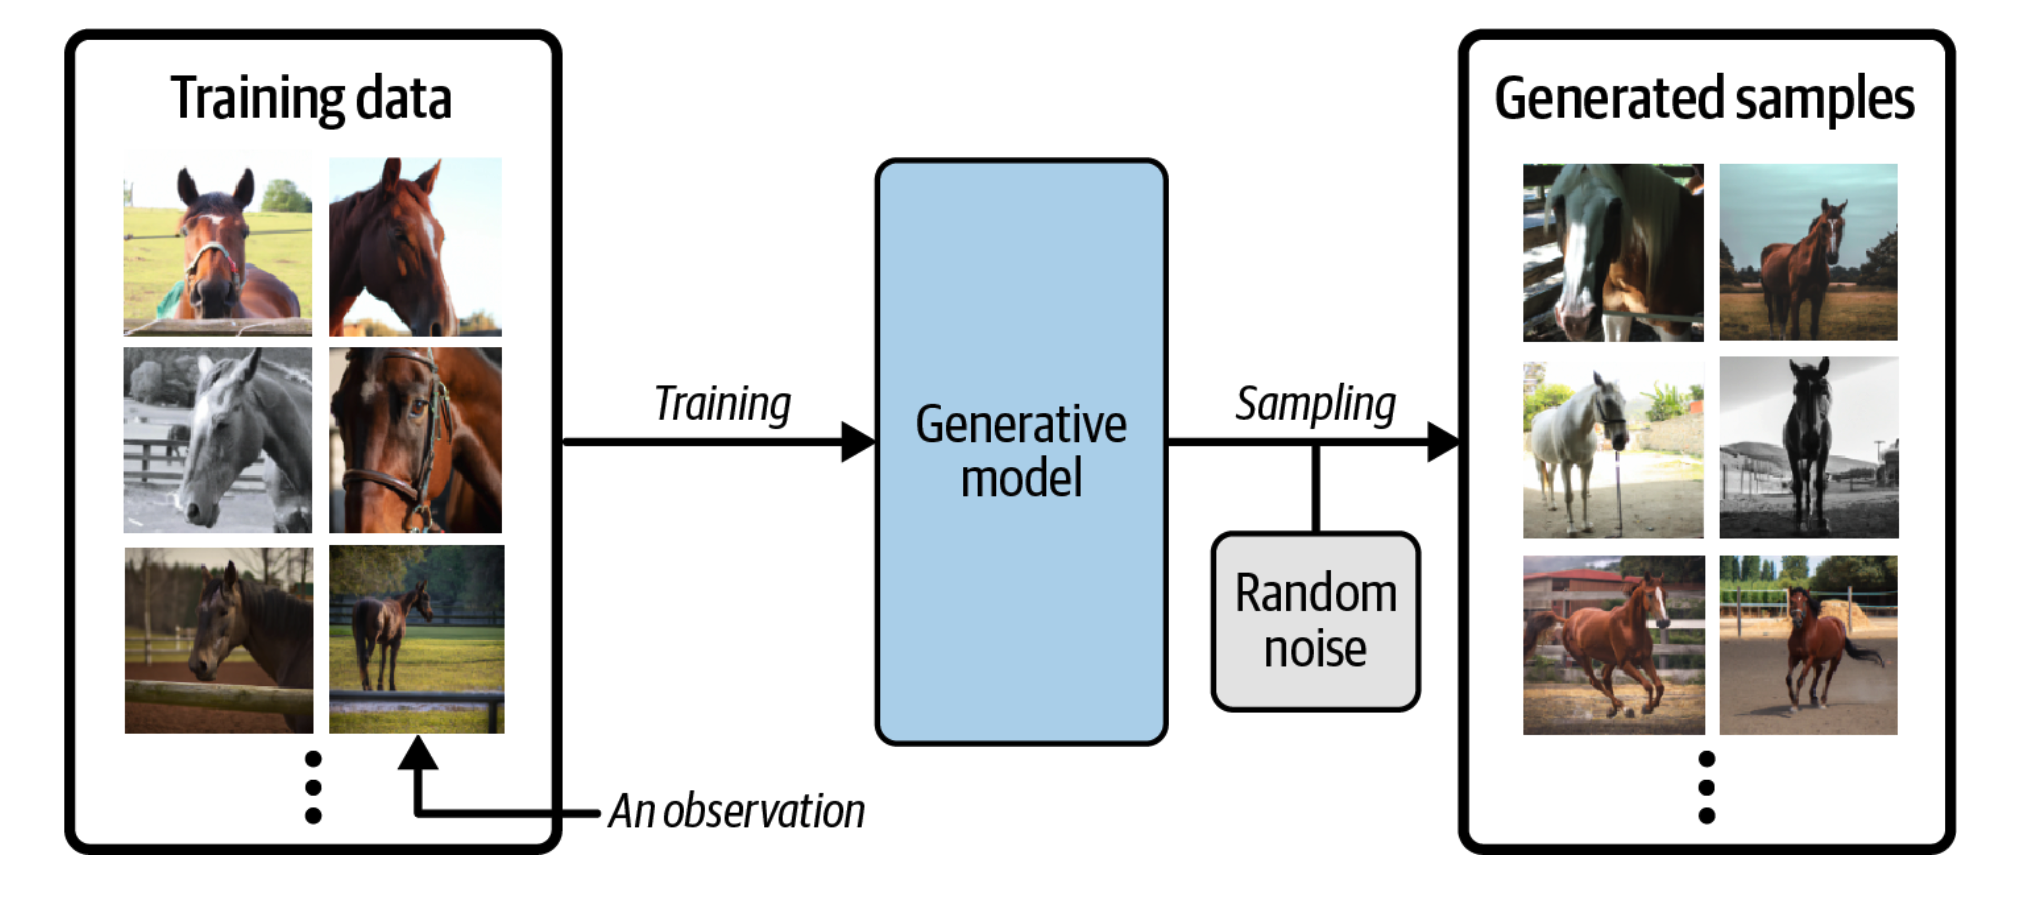
\includegraphics[width=1.0\linewidth]{figures/generativelearning.png}}

\vspace{6mm}
\end{frame}

\begin{frame}[plain,fragile]
\frametitle{Example of discriminative modeling, \href{{https://www.oreilly.com/library/view/generative-deep-learning/9781098134174/ch01.html}}{taken from Generative Deep Learning by David Foster}}

\vspace{6mm}

% inline figure
\centerline{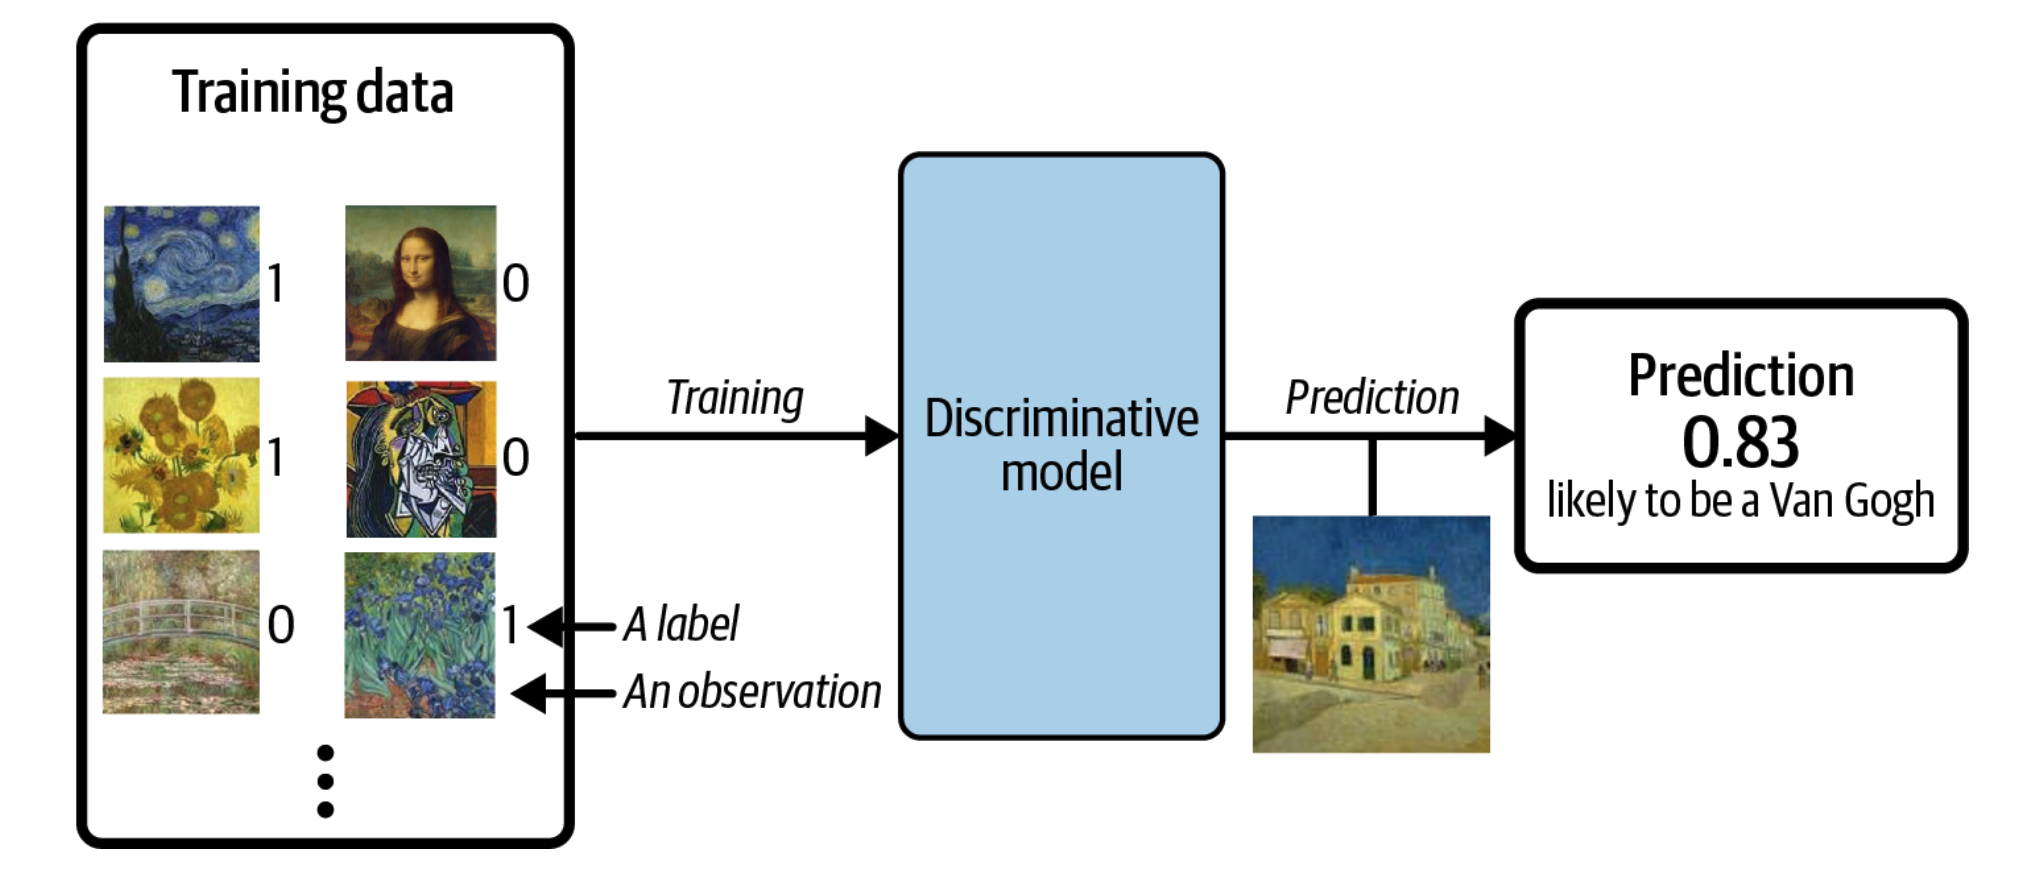
\includegraphics[width=1.0\linewidth]{figures/standarddeeplearning.png}}

\vspace{6mm}
\end{frame}

\begin{frame}[plain,fragile]
\frametitle{Taxonomy of generative deep learning, \href{{https://www.oreilly.com/library/view/generative-deep-learning/9781098134174/ch01.html}}{taken from Generative Deep Learning by David Foster}}

\vspace{6mm}

% inline figure
\centerline{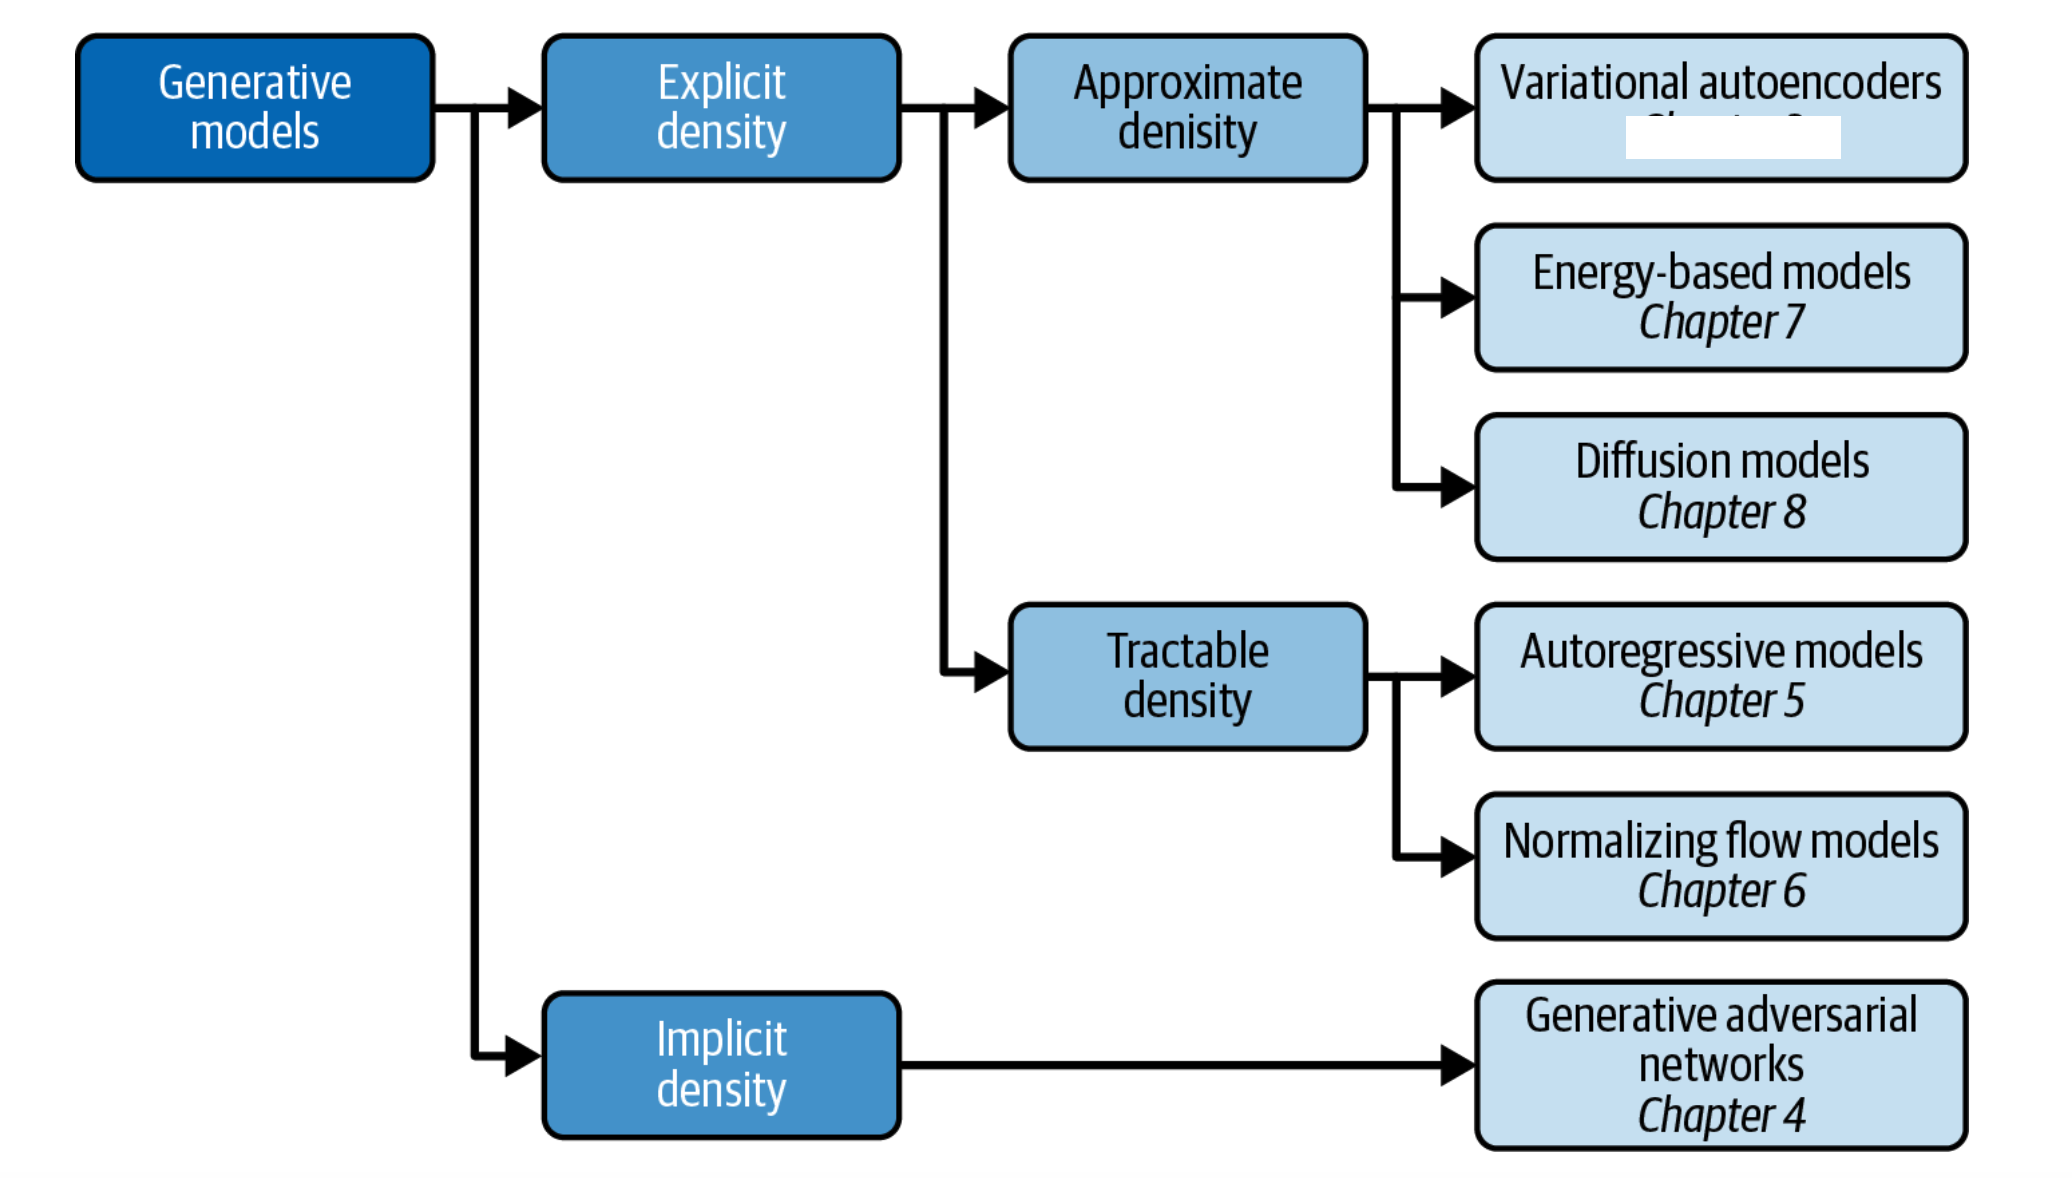
\includegraphics[width=1.0\linewidth]{figures/generativemodels.png}}

\vspace{6mm}
\end{frame}

\begin{frame}[plain,fragile]
\frametitle{Good books with hands-on material and codes}

\begin{block}{}
\begin{itemize}
\item \href{{https://sebastianraschka.com/blog/2022/ml-pytorch-book.html}}{Sebastian Rashcka et al, Machine learning with Sickit-Learn and PyTorch}

\item \href{{https://www.oreilly.com/library/view/generative-deep-learning/9781098134174/ch01.html}}{David Foster, Generative Deep Learning with TensorFlow}

\item \href{{https://github.com/PacktPublishing/Hands-On-Generative-AI-with-Python-and-TensorFlow-2}}{Bali and Gavras, Generative AI with Python and TensorFlow 2}
\end{itemize}

\noindent
\end{block}

All three books have GitHub addresses from where  one can download all codes. We will borrow most of the material from these three texts as well as 
from Goodfellow, Bengio and Courville's text \href{{https://www.deeplearningbook.org/}}{Deep Learning}
\end{frame}

\begin{frame}[plain,fragile]
\frametitle{More selected references}

\begin{block}{}
\begin{itemize}
\item \href{{https://arxiv.org/abs/1803.08823}}{Mehta et al.} and \href{{https://www.sciencedirect.com/science/article/pii/S0370157319300766?via%3Dihub}}{Physics Reports (2019)}.

\item \href{{https://link.aps.org/doi/10.1103/RevModPhys.91.045002}}{Machine Learning and the Physical Sciences by Carleo et al}

\item \href{{https://journals.aps.org/rmp/abstract/10.1103/RevModPhys.94.031003}}{Artificial Intelligence and Machine Learning in Nuclear Physics, Amber Boehnlein et al., Reviews Modern of Physics 94, 031003 (2022)} 

\item \href{{https://journals.aps.org/prresearch/pdf/10.1103/PhysRevResearch.5.033062}}{Dilute neutron star matter from neural-network quantum states by Fore et al, Physical Review Research 5, 033062 (2023)}

\item \href{{https://doi.org/10.48550/arXiv.2305.08831}}{Neural-network quantum states for ultra-cold Fermi gases, Jane Kim et al, Nature Physics Communcication, submitted}

\item \href{{https://doi.org/10.48550/arXiv.2305.07240}}{Message-Passing Neural Quantum States for the Homogeneous Electron Gas, Gabriel Pescia, Jane Kim et al.~arXiv.2305.07240,}
\end{itemize}

\noindent
\end{block}
\end{frame}

\begin{frame}[plain,fragile]
\frametitle{Lots of room for creativity}

\begin{block}{}
Not all the
algorithms and methods can be given a rigorous mathematical
justification, opening up thereby for experimenting
and trial and error and thereby exciting new developments. 
\end{block}

\begin{block}{}
A solid command of linear algebra, multivariate theory, 
probability theory, statistical data analysis, optimization algorithms, 
understanding errors and Monte Carlo methods is important in order to understand many of the 
various algorithms and methods. 
\end{block}

\textbf{Job market, a personal statement}: \href{{https://www.analyticsindiamag.com/top-countries-hiring-most-number-of-artificial-intelligence-machine-learning-experts/}}{A familiarity with ML is almost becoming a prerequisite for many of the most exciting employment opportunities}. And add quantum computing and there you are!
\end{frame}

\begin{frame}[plain,fragile]
\frametitle{Machine learning. A simple perspective on the interface between ML and Physics}

\vspace{6mm}

% inline figure
\centerline{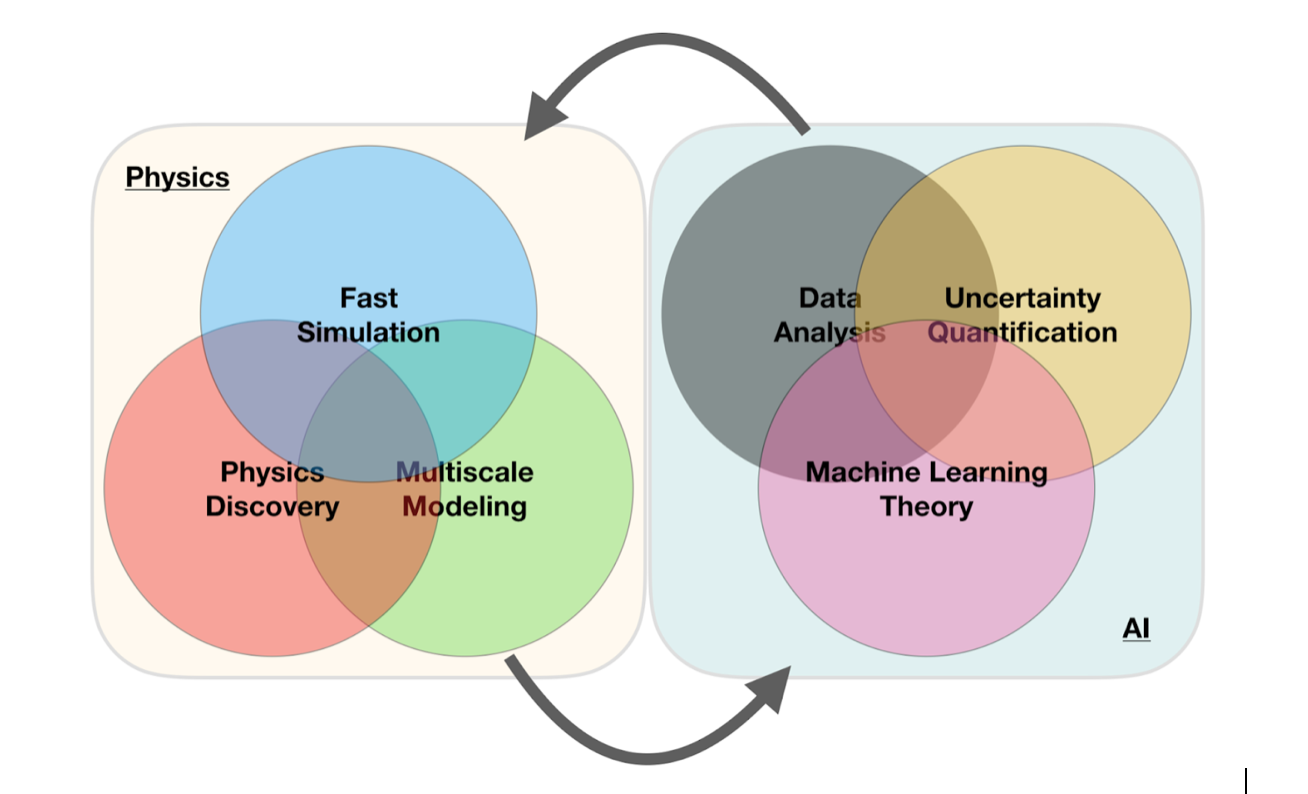
\includegraphics[width=1.0\linewidth]{figures/mlimage.png}}

\vspace{6mm}
\end{frame}

\begin{frame}[plain,fragile]
\frametitle{AI/ML and Quantum Computing}

\vspace{6mm}

% inline figure
\centerline{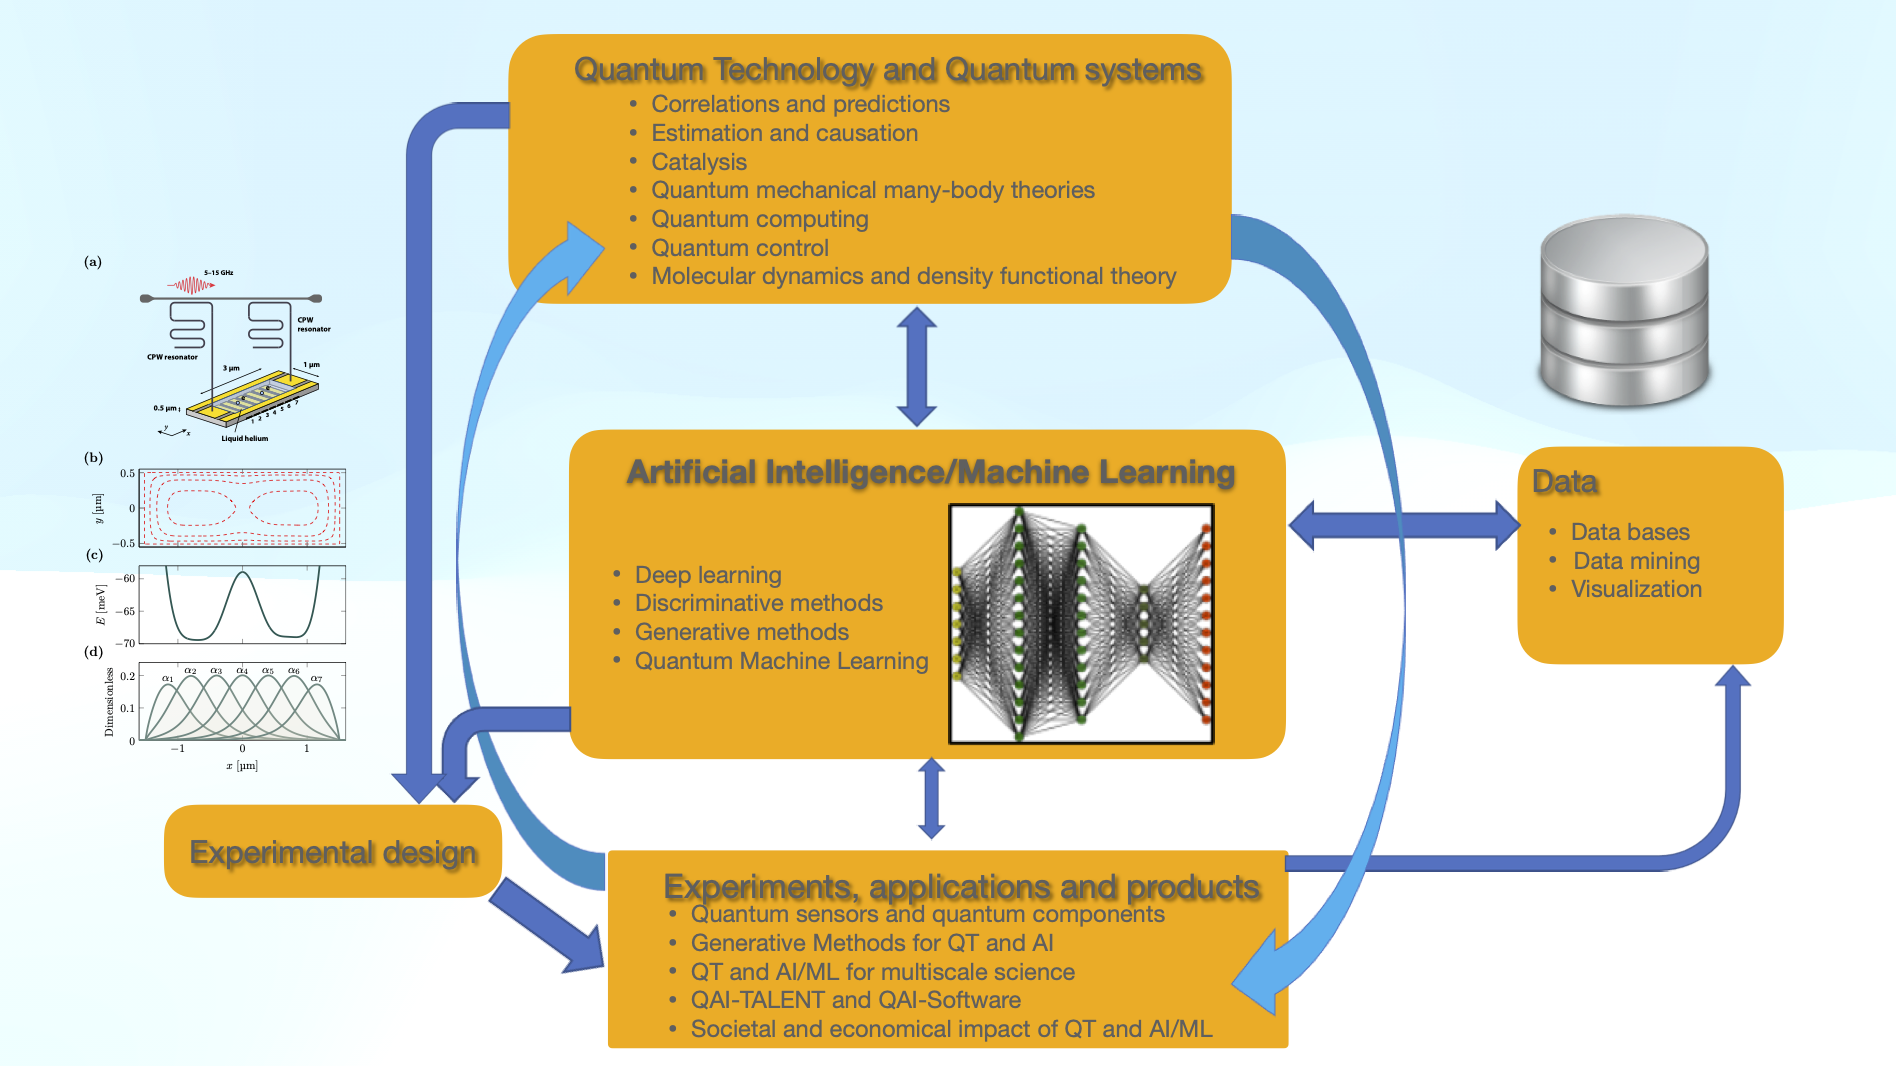
\includegraphics[width=1.0\linewidth]{figures/QAIfig1.png}}

\vspace{6mm}
\end{frame}

\begin{frame}[plain,fragile]
\frametitle{What are the basic Machine Learning ingredients?}

\begin{block}{}
Almost every problem in ML and data science starts with the same ingredients:
\begin{itemize}
\item The dataset $\bm{x}$ (could be some observable quantity of the system we are studying)

\item A model which is a function of a set of parameters $\bm{\alpha}$ that relates to the dataset, say a likelihood  function $p(\bm{x}\vert \bm{\alpha})$ or just a simple model $f(\bm{\alpha})$

\item A so-called \textbf{loss/cost/risk} function $\mathcal{C} (\bm{x}, f(\bm{\alpha}))$ which allows us to decide how well our model represents the dataset. 
\end{itemize}

\noindent
We seek to minimize the function $\mathcal{C} (\bm{x}, f(\bm{\alpha}))$ by finding the parameter values which minimize $\mathcal{C}$. This leads to  various minimization algorithms. It may surprise many, but at the heart of all machine learning algortihms there is an optimization problem. 
\end{block}
\end{frame}

\begin{frame}[plain,fragile]
\frametitle{Optimization at the heart of all ML}

\vspace{6mm}

% inline figure
\centerline{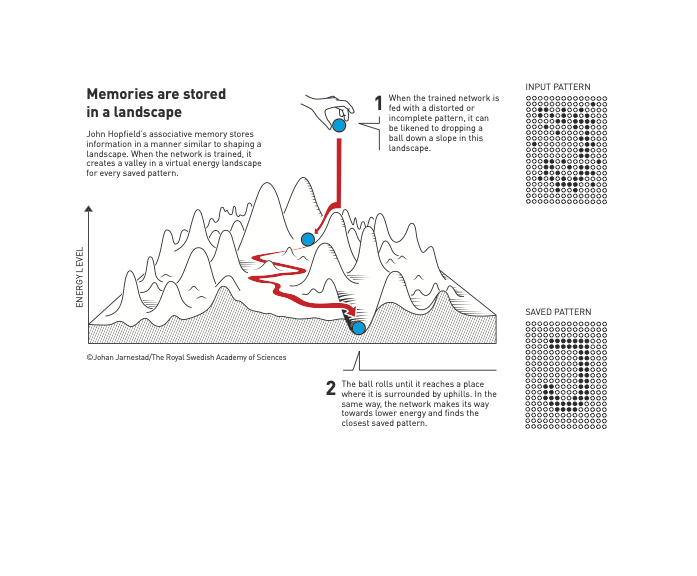
\includegraphics[width=1.0\linewidth]{figures/optimization.png}}

\vspace{6mm}
\end{frame}

\begin{frame}[plain,fragile]
\frametitle{Low-level machine learning, the family of ordinary least squares methods}

Our data which we want to apply a machine learning method on, consist
of a set of inputs $\bm{x}^T=[x_0,x_1,x_2,\dots,x_{n-1}]$ and the
outputs we want to model $\bm{y}^T=[y_0,y_1,y_2,\dots,y_{n-1}]$.
We assume  that the output data can be represented (for a regression case) by a continuous function $f$
through
\[
\bm{y}=f(\bm{x})+\bm{\epsilon}.
\]
\end{frame}

\begin{frame}[plain,fragile]
\frametitle{Setting up the equations}

In linear regression we approximate the unknown function with another
continuous function $\tilde{\bm{y}}(\bm{x})$ which depends linearly on
some unknown parameters
$\bm{\theta}^T=[\theta_0,\theta_1,\theta_2,\dots,\theta_{p-1}]$.

The input data can be organized in terms of a so-called design matrix 
with an approximating function $\bm{\tilde{y}}$ 
\[
\bm{\tilde{y}}= \bm{X}\bm{\theta},
\]
\end{frame}

\begin{frame}[plain,fragile]
\frametitle{The objective/cost/loss function}

The  simplest approach is the mean squared error
\[
C(\bm{\Theta})=\frac{1}{n}\sum_{i=0}^{n-1}\left(y_i-\tilde{y}_i\right)^2=\frac{1}{n}\left\{\left(\bm{y}-\bm{\tilde{y}}\right)^T\left(\bm{y}-\bm{\tilde{y}}\right)\right\},
\]
or using the matrix $\bm{X}$ and in a more compact matrix-vector notation as
\[
C(\bm{\Theta})=\frac{1}{n}\left\{\left(\bm{y}-\bm{X}\bm{\theta}\right)^T\left(\bm{y}-\bm{X}\bm{\theta}\right)\right\}.
\]
This function represents one of many possible ways to define the so-called cost function.
\end{frame}

\begin{frame}[plain,fragile]
\frametitle{Training solution}

Optimizing with respect to the unknown parameters $\theta_j$ we get 
\[
\bm{X}^T\bm{y} = \bm{X}^T\bm{X}\bm{\theta},  
\]
and if the matrix $\bm{X}^T\bm{X}$ is invertible we have the optimal values
\[
\hat{\bm{\theta}} =\left(\bm{X}^T\bm{X}\right)^{-1}\bm{X}^T\bm{y}.
\]

We say we 'learn' the unknown parameters $\bm{\theta}$ from the last equation.
\end{frame}

\begin{frame}[plain,fragile]
\frametitle{Inspiration from Neuroscience}

\vspace{6mm}

% inline figure
\centerline{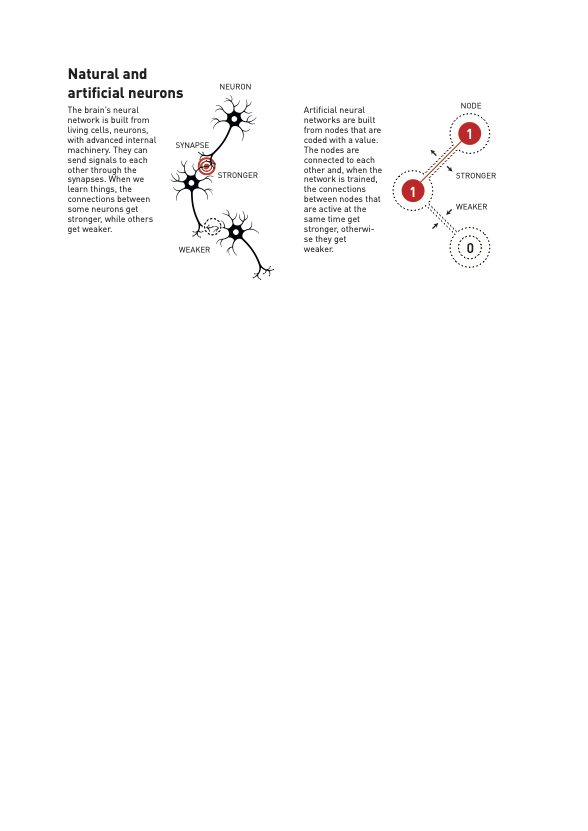
\includegraphics[width=1.0\linewidth]{figures/neuronandnn.png}}

\vspace{6mm}
\end{frame}

\begin{frame}[plain,fragile]
\frametitle{Why Feed Forward Neural Networks (FFNN)?}

According to the \emph{Universal approximation theorem}, a feed-forward
neural network with just a single hidden layer containing a finite
number of neurons can approximate a continuous multidimensional
function to arbitrary accuracy, assuming the activation function for
the hidden layer is a \textbf{non-constant, bounded and
monotonically-increasing continuous function}.
\end{frame}

\begin{frame}[plain,fragile]
\frametitle{Universal approximation theorem}

The universal approximation theorem plays a central role in deep
learning.  \href{{https://link.springer.com/article/10.1007/BF02551274}}{Cybenko (1989)} showed
the following:

\begin{block}{}
Let $\sigma$ be any continuous sigmoidal function such that
\[
\sigma(z) = \left\{\begin{array}{cc} 1 & z\rightarrow \infty\\ 0 & z \rightarrow -\infty \end{array}\right.
\]
Given a continuous and deterministic function $F(\bm{x})$ on the unit
cube in $d$-dimensions $F\in [0,1]^d$, $x\in [0,1]^d$ and a parameter
$\epsilon >0$, there is a one-layer (hidden) neural network
$f(\bm{x};\bm{\Theta})$ with $\bm{\Theta}=(\bm{W},\bm{b})$ and $\bm{W}\in
\mathbb{R}^{m\times n}$ and $\bm{b}\in \mathbb{R}^{n}$, for which
\[
\vert F(\bm{x})-f(\bm{x};\bm{\Theta})\vert < \epsilon \hspace{0.1cm} \forall \bm{x}\in[0,1]^d.
\]

\end{block}
\end{frame}

\begin{frame}[plain,fragile]
\frametitle{The approximation theorem in words}

\textbf{Any continuous function $y=F(\bm{x})$ supported on the unit cube in
$d$-dimensions can be approximated by a one-layer sigmoidal network to
arbitrary accuracy.}

\href{{https://www.sciencedirect.com/science/article/abs/pii/089360809190009T}}{Hornik (1991)} extended the theorem by letting any non-constant, bounded activation function to be included using that the expectation value
\[
\mathbb{E}[\vert F(\bm{x})\vert^2] =\int_{\bm{x}\in D} \vert F(\bm{x})\vert^2p(\bm{x})d\bm{x} < \infty.
\]
Then we have
\[
\mathbb{E}[\vert F(\bm{x})-f(\bm{x};\bm{\Theta})\vert^2] =\int_{\bm{x}\in D} \vert F(\bm{x})-f(\bm{x};\bm{\Theta})\vert^2p(\bm{x})d\bm{x} < \epsilon.
\]
\end{frame}

\begin{frame}[plain,fragile]
\frametitle{More on the general approximation theorem}

None of the proofs give any insight into the relation between the
number of of hidden layers and nodes and the approximation error
$\epsilon$, nor the magnitudes of $\bm{W}$ and $\bm{b}$.

Neural networks (NNs) have what we may call a kind of universality no matter what function we want to compute.

\begin{block}{}
It does not mean that an NN can be used to exactly compute any function. Rather, we get an approximation that is as good as we want. 
\end{block}
\end{frame}

\begin{frame}[plain,fragile]
\frametitle{Class of functions we can approximate}

\begin{block}{}
The class of functions that can be approximated are the continuous ones.
If the function $F(\bm{x})$ is discontinuous, it won't in general be possible to approximate it. However, an NN may still give an approximation even if we fail in some points.
\end{block}
\end{frame}

\begin{frame}[plain,fragile]
\frametitle{Many-body physics, Quantum Monte Carlo and deep learning}

\begin{block}{}
Given a hamiltonian $H$ and a trial wave function $\Psi_T$, the variational principle states that the expectation value of $\langle H \rangle$, defined through 
\[
   \langle E \rangle =
   \frac{\int d\bm{R}\Psi^{\ast}_T(\bm{R})H(\bm{R})\Psi_T(\bm{R})}
        {\int d\bm{R}\Psi^{\ast}_T(\bm{R})\Psi_T(\bm{R})},
\]
is an upper bound to the ground state energy $E_0$ of the hamiltonian $H$, that is 
\[
    E_0 \le \langle E \rangle.
\]
In general, the integrals involved in the calculation of various  expectation values  are multi-dimensional ones. Traditional integration methods such as the Gauss-Legendre will not be adequate for say the  computation of the energy of a many-body system.  \textbf{Basic philosophy: Let a neural network find the optimal wave function}
\end{block}
\end{frame}

\begin{frame}[plain,fragile]
\frametitle{Quantum Monte Carlo Motivation}

\begin{block}{Basic steps }
Choose a trial wave function
$\psi_T(\bm{R})$.
\[
   P(\bm{R},\bm{\alpha})= \frac{\left|\psi_T(\bm{R},\bm{\alpha})\right|^2}{\int \left|\psi_T(\bm{R},\bm{\alpha})\right|^2d\bm{R}}.
\]
This is our model, or likelihood/probability distribution function  (PDF). It depends on some variational parameters $\bm{\alpha}$.
The approximation to the expectation value of the Hamiltonian is now 
\[
   \langle E[\bm{\alpha}] \rangle = 
   \frac{\int d\bm{R}\Psi^{\ast}_T(\bm{R},\bm{\alpha})H(\bm{R})\Psi_T(\bm{R},\bm{\alpha})}
        {\int d\bm{R}\Psi^{\ast}_T(\bm{R},\bm{\alpha})\Psi_T(\bm{R},\bm{\alpha})}.
\]
\end{block}
\end{frame}

\begin{frame}[plain,fragile]
\frametitle{Quantum Monte Carlo Motivation}

\begin{block}{Define a new quantity }
\[
   E_L(\bm{R},\bm{\alpha})=\frac{1}{\psi_T(\bm{R},\bm{\alpha})}H\psi_T(\bm{R},\bm{\alpha}),
\]
called the local energy, which, together with our trial PDF yields
\[
  \langle E[\bm{\alpha}] \rangle=\int P(\bm{R})E_L(\bm{R},\bm{\alpha}) d\bm{R}\approx \frac{1}{N}\sum_{i=1}^NE_L(\bm{R_i},\bm{\alpha})
\]
with $N$ being the number of Monte Carlo samples.
\end{block}
\end{frame}

\begin{frame}[plain,fragile]
\frametitle{Energy derivatives}

\begin{block}{}
The local energy as function of the variational parameters defines now our \textbf{objective/cost} function.

To find the derivatives of the local energy expectation value as function of the variational parameters, we can use the chain rule and the hermiticity of the Hamiltonian.  

Let us define (with the notation $\langle E[\bm{\alpha}]\rangle =\langle  E_L\rangle$)
\[
\bar{E}_{\alpha_i}=\frac{d\langle  E_L\rangle}{d\alpha_i},
\]
as the derivative of the energy with respect to the variational parameter $\alpha_i$
We define also the derivative of the trial function (skipping the subindex $T$) as 
\[
\bar{\Psi}_{i}=\frac{d\Psi}{d\alpha_i}.
\]
\end{block}
\end{frame}

\begin{frame}[plain,fragile]
\frametitle{Derivatives of the local energy}

\begin{block}{}
The elements of the gradient of the local energy are 
\[
\bar{E}_{i}= 2\left( \langle \frac{\bar{\Psi}_{i}}{\Psi}E_L\rangle -\langle \frac{\bar{\Psi}_{i}}{\Psi}\rangle\langle E_L \rangle\right).
\]
From a computational point of view it means that you need to compute the expectation values of 
\[
\langle \frac{\bar{\Psi}_{i}}{\Psi}E_L\rangle,
\]
and
\[
\langle \frac{\bar{\Psi}_{i}}{\Psi}\rangle\langle E_L\rangle
\]
These integrals are evaluted using MC intergration (with all its possible error sources). Use methods like stochastic gradient or other minimization methods to find the optimal parameters.
\end{block}
\end{frame}

\begin{frame}[plain,fragile]
\frametitle{Ansatz for a fermionic state function, Jane Kim et al, Commun Phys 7, 148 (2024)}

\[
\Psi_T(\bm{X}) =\exp{U(\bm{X})}\Phi(\bm{X}).
\]

\begin{block}{}
\begin{enumerate}
\item Build in fermion antisymmetry for network compactness

\item Permutation-invariant Jastrow function improves ansatz flexibility

\item Build $U$ and $\Phi$ functions from fully connected, deep neural networks

\item Use Slater determinant (or Pfaffian) $\Phi$ to enforce antisymmetry with single particle wavefunctions represented by neural networks
\end{enumerate}

\noindent
\end{block}
\end{frame}

\begin{frame}[plain,fragile]
\frametitle{Neutron star structure}

\vspace{6mm}

% inline figure
\centerline{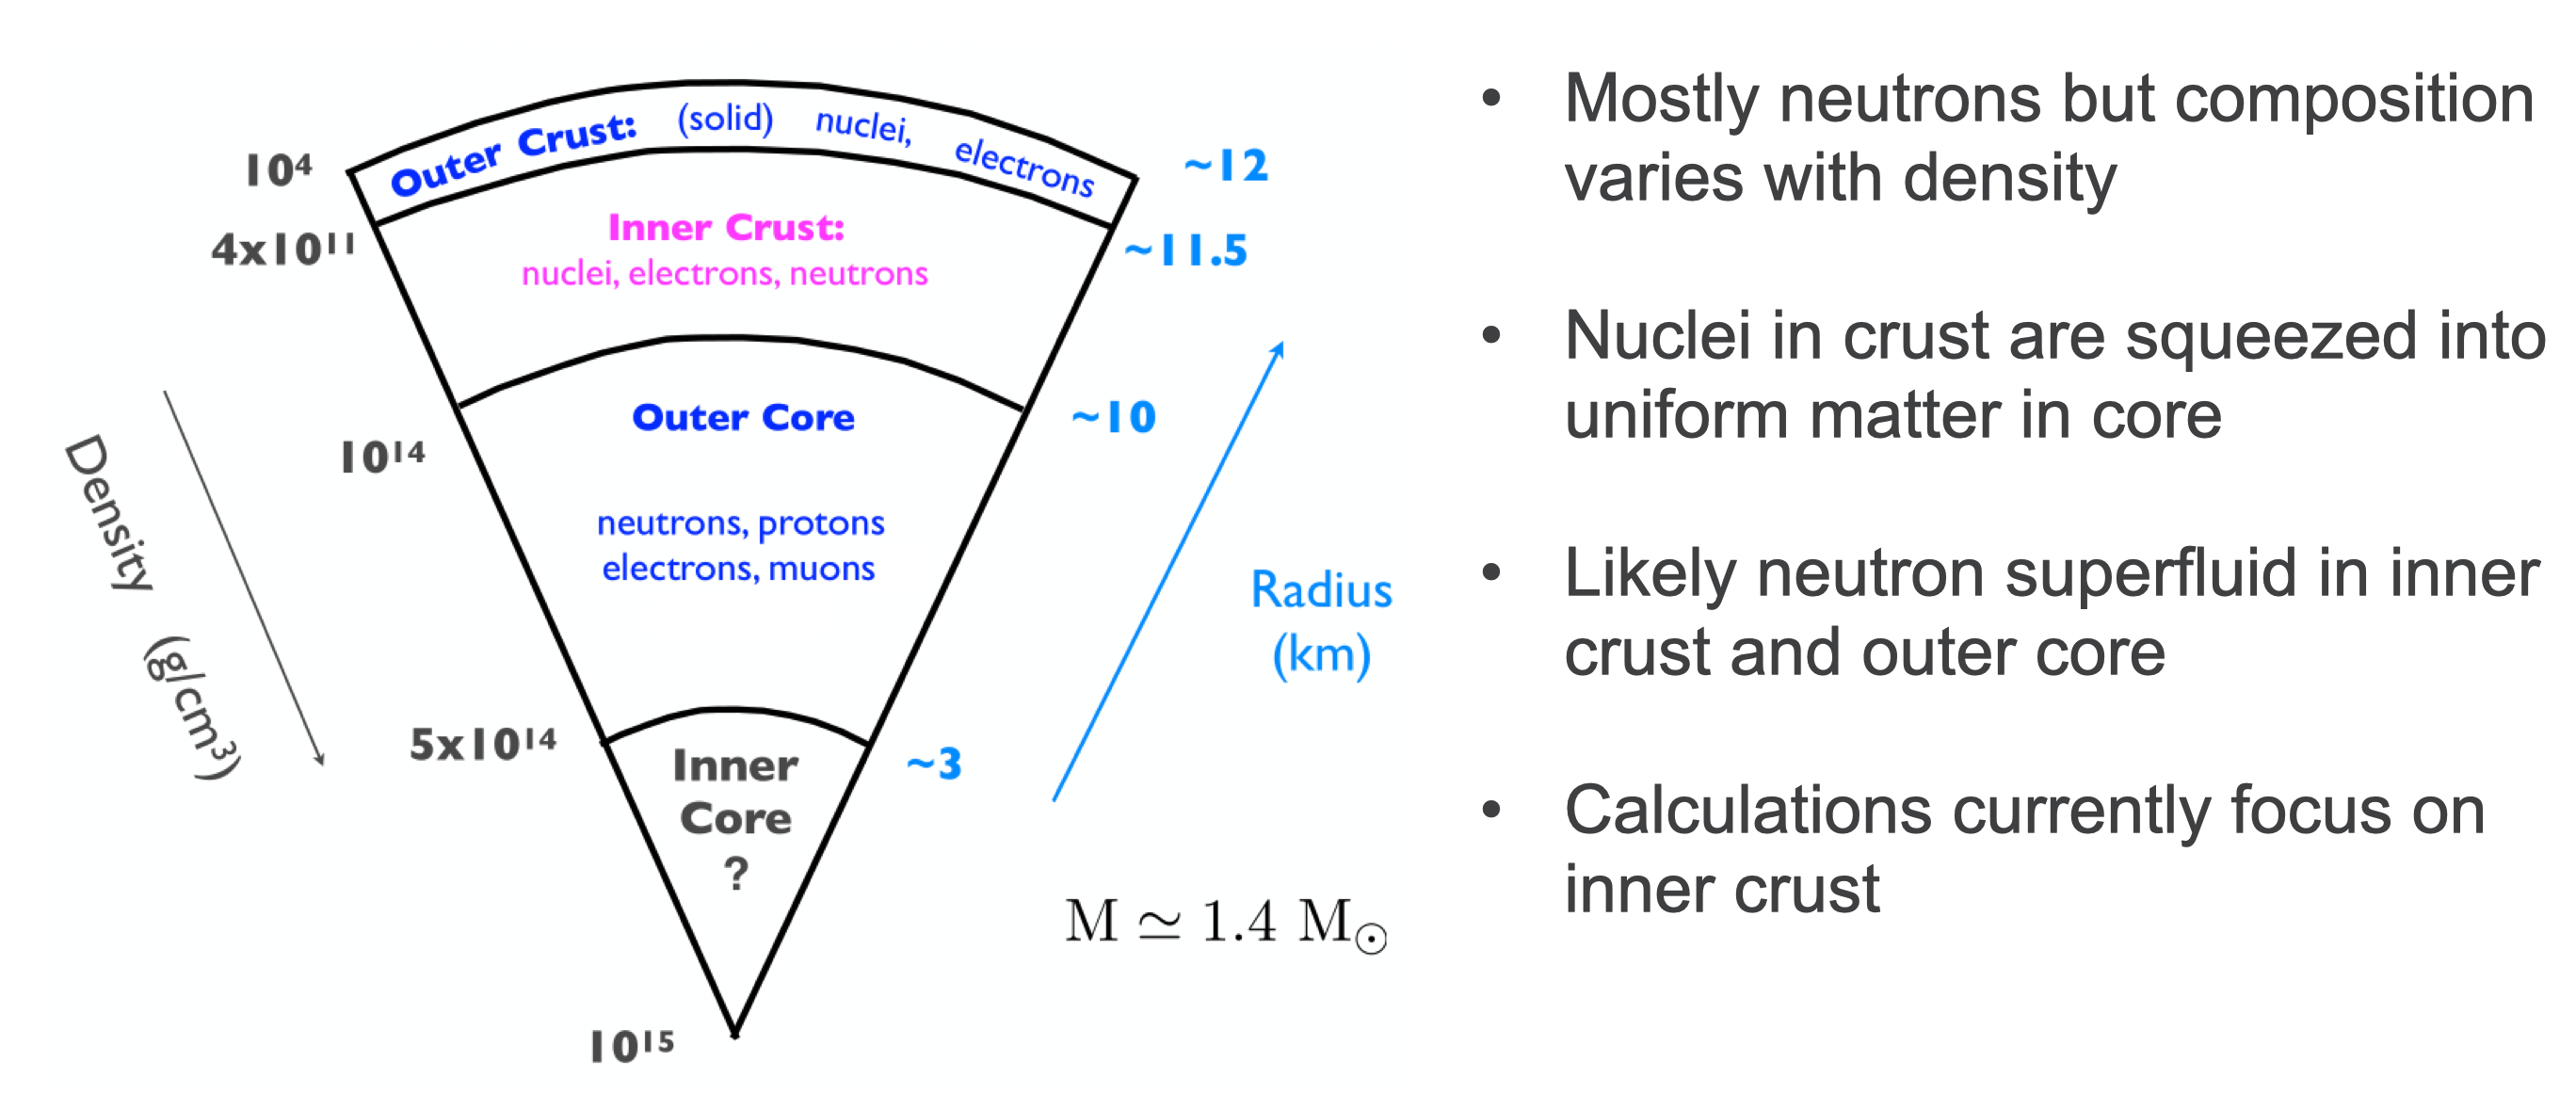
\includegraphics[width=1.0\linewidth]{figures/mbpfig5.png}}

\vspace{6mm}
\end{frame}

\begin{frame}[plain,fragile]
\frametitle{\href{{https://journals.aps.org/prresearch/pdf/10.1103/PhysRevResearch.5.033062}}{Dilute neutron star matter from neural-network quantum states by Fore et al, Physical Review Research 5, 033062 (2023)} at density $\rho=0.04$ fm$^{-3}$}

\begin{block}{}

\vspace{6mm}

% inline figure
\centerline{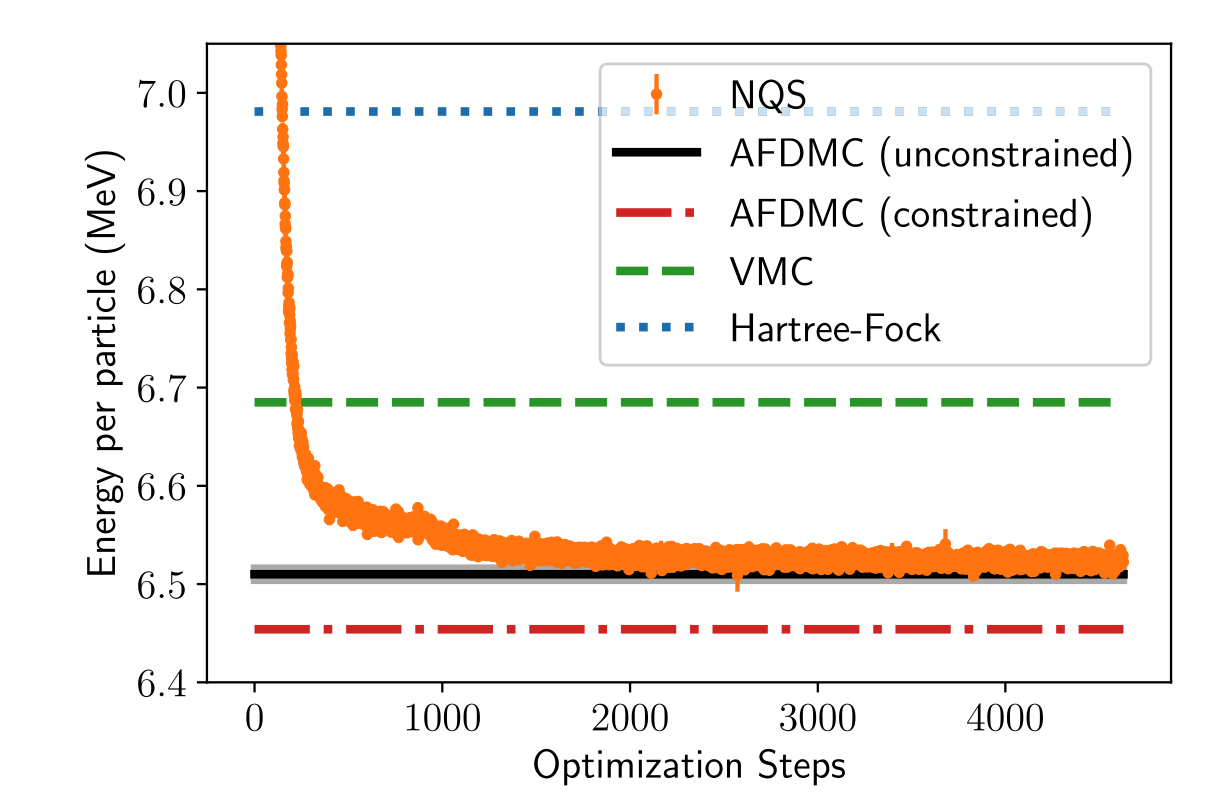
\includegraphics[width=0.9\linewidth]{figures/nmatter.png}}

\vspace{6mm}

\end{block}
\end{frame}

\begin{frame}[plain,fragile]
\frametitle{The electron gas in three dimensions with $N=14$ electrons (Wigner-Seitz radius $r_s=2$ a.u.), \href{{https://doi.org/10.48550/arXiv.2305.07240}}{Gabriel Pescia, Jane Kim et al.~arXiv.2305.07240,}}

\begin{block}{}

\vspace{6mm}

% inline figure
\centerline{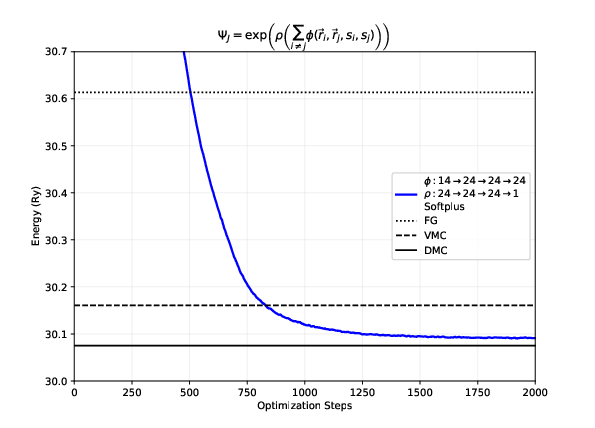
\includegraphics[width=0.9\linewidth]{figures/elgasnew.png}}

\vspace{6mm}

\end{block}
\end{frame}

\begin{frame}[plain,fragile]
\frametitle{Adesso le macchine di Boltzmann, modello basato sul lavoro di Hinton}

\vspace{6mm}

% inline figure
\centerline{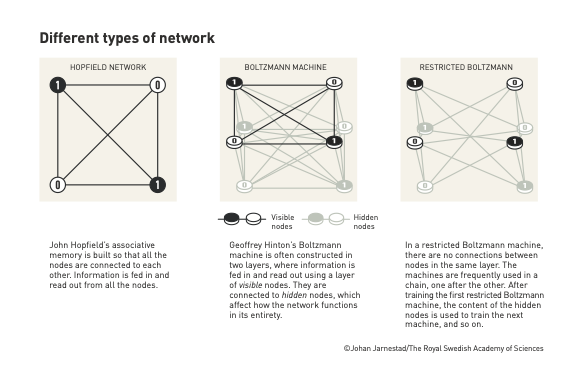
\includegraphics[width=1.0\linewidth]{figures/boltzmannnobel.png}}

\vspace{6mm}
\end{frame}

\begin{frame}[plain,fragile]
\frametitle{Essential elements of generative models}

The aim of generative methods is to train a probability distribution $p$. Popular methods are:
\begin{enumerate}
\item Energy based models, with the family of Boltzmann distributions as a typical example

\item Variational autoencoders

\item Generative adversarial networks (GANs) and

\item Diffusion models
\end{enumerate}

\noindent
\end{frame}

\begin{frame}[plain,fragile]
\frametitle{Generative models: Why Boltzmann machines?}

What is known as restricted Boltzmann Machines (RMB) have received a
lot of attention lately.  One of the major reasons is that they can be
stacked layer-wise to build deep neural networks that capture
complicated statistics.

The original RBMs had just one visible layer and a hidden layer, but
recently so-called Gaussian-binary RBMs have gained quite some
popularity in imaging since they are capable of modeling continuous
data that are common to natural images.

Furthermore, they have been used to solve complicated quantum
mechanical many-particle problems or classical statistical physics
problems like the Ising and Potts classes of models.
\end{frame}

\begin{frame}[plain,fragile]
\frametitle{The structure of the RBM network}

\vspace{6mm}

% inline figure
\centerline{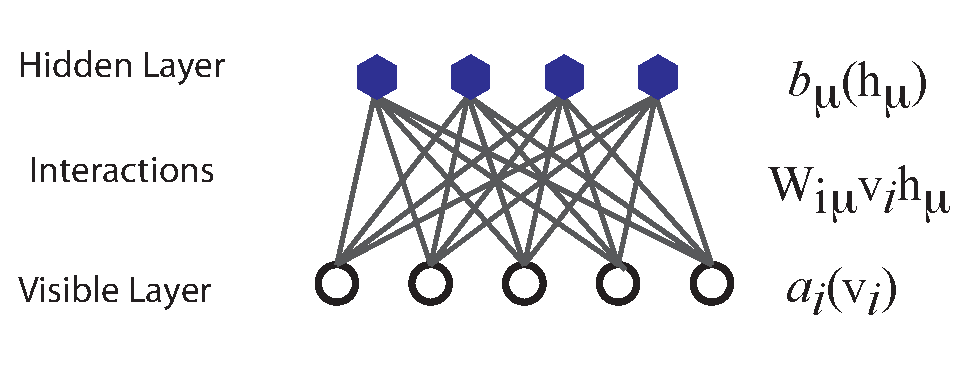
\includegraphics[width=1.0\linewidth]{figures/RBM.pdf}}

\vspace{6mm}
\end{frame}

\begin{frame}[plain,fragile]
\frametitle{The network}

\textbf{The network layers}:
\begin{enumerate}
\item A function $\bm{x}$ that represents the visible layer, a vector of $M$ elements (nodes). This layer represents both what the RBM might be given as training input, and what we want it to be able to reconstruct. This might for example be the pixels of an image, the spin values of the Ising model, or coefficients representing speech.

\item The function $\bm{h}$ represents the hidden, or latent, layer. A vector of $N$ elements (nodes). Also called "feature detectors".
\end{enumerate}

\noindent
\end{frame}

\begin{frame}[plain,fragile]
\frametitle{Goals}

The goal of the hidden layer is to increase the model's expressive
power. We encode complex interactions between visible variables by
introducing additional, hidden variables that interact with visible
degrees of freedom in a simple manner, yet still reproduce the complex
correlations between visible degrees in the data once marginalized
over (integrated out).

\textbf{The network parameters, to be optimized/learned}:
\begin{enumerate}
 \item $\bm{a}$ represents the visible bias, a vector of same length as $\bm{x}$.

 \item $\bm{b}$ represents the hidden bias, a vector of same lenght as $\bm{h}$.

 \item $W$ represents the interaction weights, a matrix of size $M\times N$.
\end{enumerate}

\noindent
\end{frame}

\begin{frame}[plain,fragile]
\frametitle{Joint distribution}

The restricted Boltzmann machine is described by a Bolztmann distribution
\[
	P_{\mathrm{rbm}}(\bm{x},\bm{h}) = \frac{1}{Z} \exp{-E(\bm{x},\bm{h})},
\]
where $Z$ is the normalization constant or partition function, defined as 
\[
	Z = \int \int \exp{-E(\bm{x},\bm{h})} d\bm{x} d\bm{h}.
\]
Note the absence of the inverse temperature in these equations.
\end{frame}

\begin{frame}[plain,fragile]
\frametitle{Network Elements, the energy function}

The function $E(\bm{x},\bm{h})$ gives the \textbf{energy} of a
configuration (pair of vectors) $(\bm{x}, \bm{h})$. The lower
the energy of a configuration, the higher the probability of it. This
function also depends on the parameters $\bm{a}$, $\bm{b}$ and
$W$. Thus, when we adjust them during the learning procedure, we are
adjusting the energy function to best fit our problem.
\end{frame}

\begin{frame}[plain,fragile]
\frametitle{Energy models}

We define a domain $\bm{X}$ of stochastic variables $\bm{X}= \{x_0,x_1, \dots , x_{n-1}\}$ with a pertinent probability distribution
\[
p(\bm{X})=\prod_{x_i\in \bm{X}}p(x_i),
\]
where we have assumed that the random varaibles $x_i$ are all independent and identically distributed (iid).

We will now assume that we can defined this function in terms of optimization parameters $\bm{\Theta}$, which could be the biases and weights of a deep network, and a set of hidden variables we also assume to be random variables which also are iid. The domain of these variables is
$\bm{H}= \{h_0,h_1, \dots , h_{m-1}\}$.
\end{frame}

\begin{frame}[plain,fragile]
\frametitle{Probability model}

We define a probability
\[
p(x_i,h_j;\bm{\Theta}) = \frac{f(x_i,h_j;\bm{\Theta})}{Z(\bm{\Theta})},
\]
where $f(x_i,h_j;\bm{\Theta})$ is a function which we assume is larger or
equal than zero and obeys all properties required for a probability
distribution and $Z(\bm{\Theta})$ is a normalization constant. Inspired by
statistical mechanics, we call it often for the partition function.
It is defined as (assuming that we have discrete probability distributions)
\[
Z(\bm{\Theta})=\sum_{x_i\in \bm{X}}\sum_{h_j\in \bm{H}} f(x_i,h_j;\bm{\Theta}).
\]
\end{frame}

\begin{frame}[plain,fragile]
\frametitle{Marginal and conditional probabilities}

We can in turn define the marginal probabilities
\[
p(x_i;\bm{\Theta}) = \frac{\sum_{h_j\in \bm{H}}f(x_i,h_j;\bm{\Theta})}{Z(\bm{\Theta})},
\]
and 
\[
p(h_i;\bm{\Theta}) = \frac{\sum_{x_i\in \bm{X}}f(x_i,h_j;\bm{\Theta})}{Z(\bm{\Theta})}.
\]
\end{frame}

\begin{frame}[plain,fragile]
\frametitle{Change of notation}

\textbf{Note the change to a vector notation}. A variable like $\bm{x}$
represents now a specific \textbf{configuration}. We can generate an infinity
of such configurations. The final partition function is then the sum
over all such possible configurations, that is

\[
Z(\bm{\Theta})=\sum_{x_i\in \bm{X}}\sum_{h_j\in \bm{H}} f(x_i,h_j;\bm{\Theta}),
\]
changes to
\[
Z(\bm{\Theta})=\sum_{\bm{x}}\sum_{\bm{h}} f(\bm{x},\bm{h};\bm{\Theta}).
\]
If we have a binary set of variable $x_i$ and $h_j$ and $M$ values of $x_i$ and $N$ values of $h_j$ we have in total $2^M$ and $2^N$ possible $\bm{x}$ and $\bm{h}$ configurations, respectively.

We see that even for the modest binary case, we can easily approach a
number of configuration which is not possible to deal with.
\end{frame}

\begin{frame}[plain,fragile]
\frametitle{Optimization problem}

At the end, we are not interested in the probabilities of the hidden variables. The probability we thus want to optimize is 
\[
p(\bm{X};\bm{\Theta})=\prod_{x_i\in \bm{X}}p(x_i;\bm{\Theta})=\prod_{x_i\in \bm{X}}\left(\frac{\sum_{h_j\in \bm{H}}f(x_i,h_j;\bm{\Theta})}{Z(\bm{\Theta})}\right),
\]
which we rewrite as
\[
p(\bm{X};\bm{\Theta})=\frac{1}{Z(\bm{\Theta})}\prod_{x_i\in \bm{X}}\left(\sum_{h_j\in \bm{H}}f(x_i,h_j;\bm{\Theta})\right).
\]
\end{frame}

\begin{frame}[plain,fragile]
\frametitle{Further simplifications}

We simplify further by rewriting it as
\[
p(\bm{X};\bm{\Theta})=\frac{1}{Z(\bm{\Theta})}\prod_{x_i\in \bm{X}}f(x_i;\bm{\Theta}),
\]
where we used $p(x_i;\bm{\Theta}) = \sum_{h_j\in \bm{H}}f(x_i,h_j;\bm{\Theta})$.
The optimization problem is then
\[
{\displaystyle \mathrm{arg} \hspace{0.1cm}\max_{\bm{\bm{\Theta}}\in {\mathbb{R}}^{p}}} \hspace{0.1cm}p(\bm{X};\bm{\Theta}).
\]
\end{frame}

\begin{frame}[plain,fragile]
\frametitle{Optimizing the logarithm instead}

Computing the derivatives with respect to the parameters $\bm{\Theta}$ is
easier (and equivalent) with taking the logarithm of the
probability. We will thus optimize
\[
{\displaystyle \mathrm{arg} \hspace{0.1cm}\max_{\bm{\bm{\Theta}}\in {\mathbb{R}}^{p}}} \hspace{0.1cm}\log{p(\bm{X};\bm{\Theta})},
\]
which leads to
\[
\nabla_{\bm{\Theta}}\log{p(\bm{X};\bm{\Theta})}=0.
\]
\end{frame}

\begin{frame}[plain,fragile]
\frametitle{Expression for the gradients}

This leads to the following equation
\[
\nabla_{\bm{\Theta}}\log{p(\bm{X};\bm{\Theta})}=\nabla_{\bm{\Theta}}\left(\sum_{x_i\in \bm{X}}\log{f(x_i;\bm{\Theta})}\right)-\nabla_{\bm{\Theta}}\log{Z(\bm{\Theta})}=0.
\]

The first term is called the positive phase and we assume that we have a model for the function $f$ from which we can sample values. Below we will develop an explicit model for this.
The second term is called the negative phase and is the one which leads to more difficulties.
\end{frame}

\begin{frame}[plain,fragile]
\frametitle{The derivative of the partition function}

The partition function, defined above as
\[
Z(\bm{\Theta})=\sum_{x_i\in \bm{X}}\sum_{h_j\in \bm{H}} f(x_i,h_j;\bm{\Theta}),
\]
is in general the most problematic term. In principle both $x$ and $h$ can span large degrees of freedom, if not even infinitely many ones, and computing the partition function itself is often not desirable or even feasible. The above derivative of the partition function can however be written in terms of an expectation value which is in turn evaluated  using Monte Carlo sampling and the theory of Markov chains, popularly shortened to MCMC (or just MC$^2$).
\end{frame}

\begin{frame}[plain,fragile]
\frametitle{Explicit expression for the derivative}

We can rewrite
\[
\nabla_{\bm{\Theta}}\log{Z(\bm{\Theta})}=\frac{\nabla_{\bm{\Theta}}Z(\bm{\Theta})}{Z(\bm{\Theta})},
\]
which reads in more detail
\[
\nabla_{\bm{\Theta}}\log{Z(\bm{\Theta})}=\frac{\nabla_{\bm{\Theta}} \sum_{x_i\in \bm{X}}f(x_i;\bm{\Theta})   }{Z(\bm{\Theta})}.
\]

We can rewrite the function $f$ (we have assumed that is larger or
equal than zero) as $f=\exp{\log{f}}$. We can then reqrite the last
equation as

\[
\nabla_{\bm{\Theta}}\log{Z(\bm{\Theta})}=\frac{ \sum_{x_i\in \bm{X}} \nabla_{\bm{\Theta}}\exp{\log{f(x_i;\bm{\Theta})}}   }{Z(\bm{\Theta})}.
\]
\end{frame}

\begin{frame}[plain,fragile]
\frametitle{Final expression}

Taking the derivative gives us
\[
\nabla_{\bm{\Theta}}\log{Z(\bm{\Theta})}=\frac{ \sum_{x_i\in \bm{X}}f(x_i;\bm{\Theta}) \nabla_{\bm{\Theta}}\log{f(x_i;\bm{\Theta})}   }{Z(\bm{\Theta})}, 
\]
which is the expectation value of $\log{f}$
\[
\nabla_{\bm{\Theta}}\log{Z(\bm{\Theta})}=\sum_{x_i\in \bm{X}}p(x_i;\bm{\Theta}) \nabla_{\bm{\Theta}}\log{f(x_i;\bm{\Theta})},
\]
that is
\[
\nabla_{\bm{\Theta}}\log{Z(\bm{\Theta})}=\mathbb{E}(\log{f(x_i;\bm{\Theta})}).
\]

This quantity is evaluated using Monte Carlo sampling, with Gibbs
sampling as the standard sampling rule.  Before we discuss the
explicit algorithms, we need to remind ourselves about Markov chains
and sampling rules like the Metropolis-Hastings algorithm and Gibbs
sampling.
\end{frame}

\begin{frame}[plain,fragile]
\frametitle{Defining different types of RBMs (Energy based models)}

There are different variants of RBMs, and the differences lie in the types of visible and hidden units we choose as well as in the implementation of the energy function $E(\bm{x},\bm{h})$. The connection between the nodes in the two layers is given by the weights $w_{ij}$. 

\begin{block}{Binary-Binary RBM: }

RBMs were first developed using binary units in both the visible and hidden layer. The corresponding energy function is defined as follows:
\[
	E(\bm{x}, \bm{h}) = - \sum_i^M x_i a_i- \sum_j^N b_j h_j - \sum_{i,j}^{M,N} x_i w_{ij} h_j,
\]
where the binary values taken on by the nodes are most commonly 0 and 1.
\end{block}
\end{frame}

\begin{frame}[plain,fragile]
\frametitle{Gaussian binary}

\begin{block}{Gaussian-Binary RBM: }

Another varient is the RBM where the visible units are Gaussian while the hidden units remain binary:
\[
	E(\bm{x}, \bm{h}) = \sum_i^M \frac{(x_i - a_i)^2}{2\sigma_i^2} - \sum_j^N b_j h_j - \sum_{i,j}^{M,N} \frac{x_i w_{ij} h_j}{\sigma_i^2}. 
\]
\end{block}
\end{frame}

\begin{frame}[plain,fragile]
\frametitle{Representing the wave function}

The wavefunction should be a probability amplitude depending on
 $\bm{x}$. The RBM model is given by the joint distribution of
 $\bm{x}$ and $\bm{h}$

\[
        P_{\mathrm{rbm}}(\bm{x},\bm{h}) = \frac{1}{Z} \exp{-E(\bm{x},\bm{h})}.
\]

To find the marginal distribution of $\bm{x}$ we set:

\[
        P_{\mathrm{rbm}}(\bm{x}) =\frac{1}{Z}\sum_{\bm{h}} \exp{-E(\bm{x}, \bm{h})}.
\]

Now this is what we use to represent the wave function, calling it a neural-network quantum state (NQS)
\[
        \vert\Psi (\bm{X})\vert^2 = P_{\mathrm{rbm}}(\bm{x}).
\]
\end{frame}

\begin{frame}[plain,fragile]
\frametitle{Define the cost function}

Now we don't necessarily have training data (unless we generate it by
using some other method). However, what we do have is the variational
principle which allows us to obtain the ground state wave function by
minimizing the expectation value of the energy of a trial wavefunction
(corresponding to the untrained NQS). Similarly to the traditional
variational Monte Carlo method then, it is the local energy we wish to
minimize. The gradient to use for the stochastic gradient descent
procedure is

\[
	C_i = \frac{\partial \langle E_L \rangle}{\partial \theta_i}
	= 2(\langle E_L \frac{1}{\Psi}\frac{\partial \Psi}{\partial \theta_i} \rangle - \langle E_L \rangle \langle \frac{1}{\Psi}\frac{\partial \Psi}{\partial \theta_i} \rangle ),
\]
where the local energy is given by
\[
	E_L = \frac{1}{\Psi} \hat{\bm{H}} \Psi.
\]
\end{frame}

\begin{frame}[plain,fragile]
\frametitle{Quantum dots and Boltzmann machines, onebody densities $N=6$, $\hbar\omega=0.1$ a.u.}

\begin{block}{}

\vspace{6mm}

% inline figure
\centerline{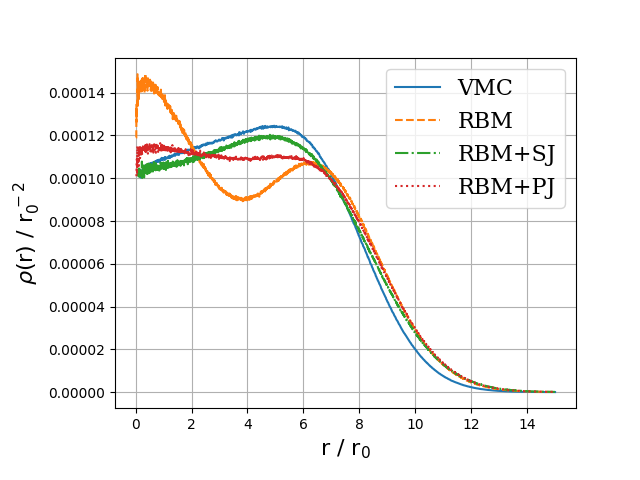
\includegraphics[width=0.9\linewidth]{figures/OB6hw01.png}}

\vspace{6mm}

\end{block}
\end{frame}

\begin{frame}[plain,fragile]
\frametitle{Onebody densities $N=30$, $\hbar\omega=1.0$ a.u.}

\begin{block}{}

\vspace{6mm}

% inline figure
\centerline{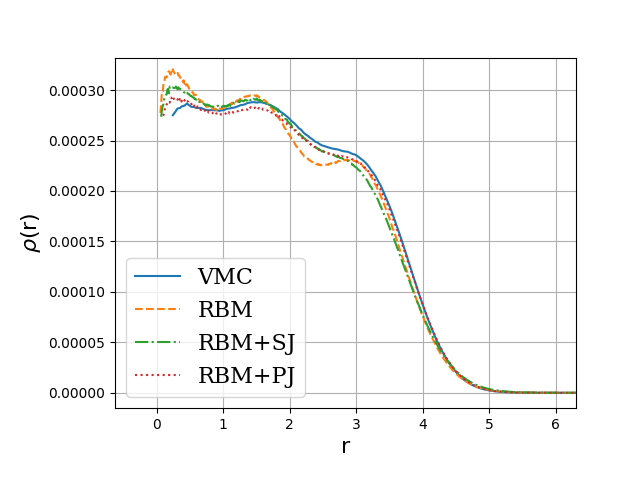
\includegraphics[width=0.9\linewidth]{figures/OB30hw1.png}}

\vspace{6mm}

\end{block}
\end{frame}

\begin{frame}[plain,fragile]
\frametitle{Expectation values as functions of the oscillator frequency}

\begin{block}{}

\vspace{6mm}

% inline figure
\centerline{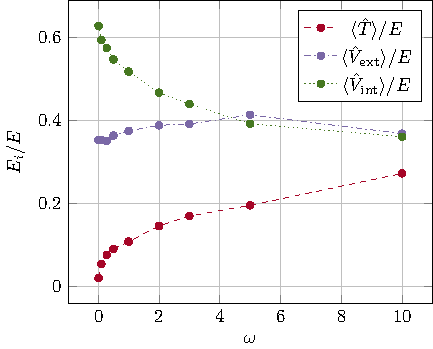
\includegraphics[width=0.9\linewidth]{figures/virialtheorem.pdf}}

\vspace{6mm}

\end{block}
\end{frame}

\begin{frame}[plain,fragile]
\frametitle{Observations (or conclusions if you prefer)}

\begin{block}{}
\begin{itemize}
\item Need for AI/Machine Learning in physics, lots of ongoing activities

\item To solve many complex problems and facilitate discoveries, multidisciplinary efforts efforts are required involving scientists in  physics, statistics, computational science, applied math and other fields.

\item There is a need for  focused AI/ML learning efforts that will benefit accelerator science and experimental and theoretical programs
\end{itemize}

\noindent
\end{block}
\end{frame}

\begin{frame}[plain,fragile]
\frametitle{More observations}

\begin{block}{}
\begin{itemize}
\item How do we develop insights, competences, knowledge in statistical learning that can advance a given field?
\begin{itemize}

  \item For example: Can we use ML to find out which correlations are relevant and thereby diminish the dimensionality problem in standard many-body  theories?

  \item Can we use AI/ML in detector analysis, accelerator design, analysis of experimental data and more?

  \item Can we use AL/ML to carry out reliable extrapolations by using current experimental knowledge and current theoretical models?

\end{itemize}

\noindent
\item The community needs to invest in relevant educational efforts and training of scientists with knowledge in AI/ML. These are great challenges to the CS and DS communities

\item Quantum computing and quantum machine learning not discussed here

\item Most likely tons of things I have forgotten
\end{itemize}

\noindent
\end{block}
\end{frame}

\begin{frame}[plain,fragile]
\frametitle{Possible start to raise awareness about ML in your own field}

\begin{block}{}
\begin{itemize}
\item Make an ML challenge in your own field a la \href{{https://home.cern/news/news/computing/higgs-boson-machine-learning-challenge}}{Learning to discover: the Higgs boson machine learning challenge}. Alternatively go to kaggle.com at \href{{https://www.kaggle.com/c/higgs-boson}}{\nolinkurl{https://www.kaggle.com/c/higgs-boson}}

\item HEP@CERN and HEP in general have made significant impacts in the field of machine learning and AI. Something to learn from
\end{itemize}

\noindent
\end{block}
\end{frame}

\begin{frame}[plain,fragile]
\frametitle{Possible questions for discussions}

\begin{enumerate}
\item How do we incorporate these topics in our education?

\item More difficult: what are the consequences for universities and our educational mission?
\end{enumerate}

\noindent
\end{frame}

\end{document}
